\chapter{Behold The Mighty Sine Wave}

\section{Anatomy of a Sine Wave}

Probably the first time you heard of the sine function was in a 
trigonometry class. You learned that if you have a right triangle, then the
sine of one of its angles was the length of the opposite size divided by
the hypotenuse (see Figure~\ref{fig_triangle}).

\begin{figure}[htbp]
\centering
\includegraphics[width=5.5in, trim=0in 3in 0in 1.5in, clip]{triangle.pdf}
\caption{In trigonometry, the sine is the opposite side of a right 
triangle divided by the hypotenuse.}
\label{fig_triangle}
\end{figure}

Maybe later in analytic geometry you saw how you can extend the definition 
of the sine function
to angles greater than $90^\circ$ or less than $0^\circ$, as in 
Figure~\ref{fig_triangle_graph}. $sin(0^\circ) = 0$ and increases until
$sin(90^\circ) = 1$. Then in falls back down to zero at $180^\circ$.
The between $180^\circ$ and $360^\circ$ it does the same thing, except
that it is negative because $y \leq 0$. For $\theta > 360^\circ$, the
angles just keep going around again and the pattern repeats.

\begin{figure}[htbp]
\centering
\includegraphics[width=5.5in, trim=0in 0.9in 0in 0.9in, clip]{triangle_graph.pdf}
\caption{In analytic geometry you can define $sin(\theta) = y/r$.}
\label{fig_triangle_graph}
\end{figure}

You can plot the sine function as in Figure~\ref{fig_sine_plot}. It is 
a graceful curve that oscillates up and down forever. half of the time
is is above zero and half of the time it is below.

\begin{figure}[htbp]
\centering
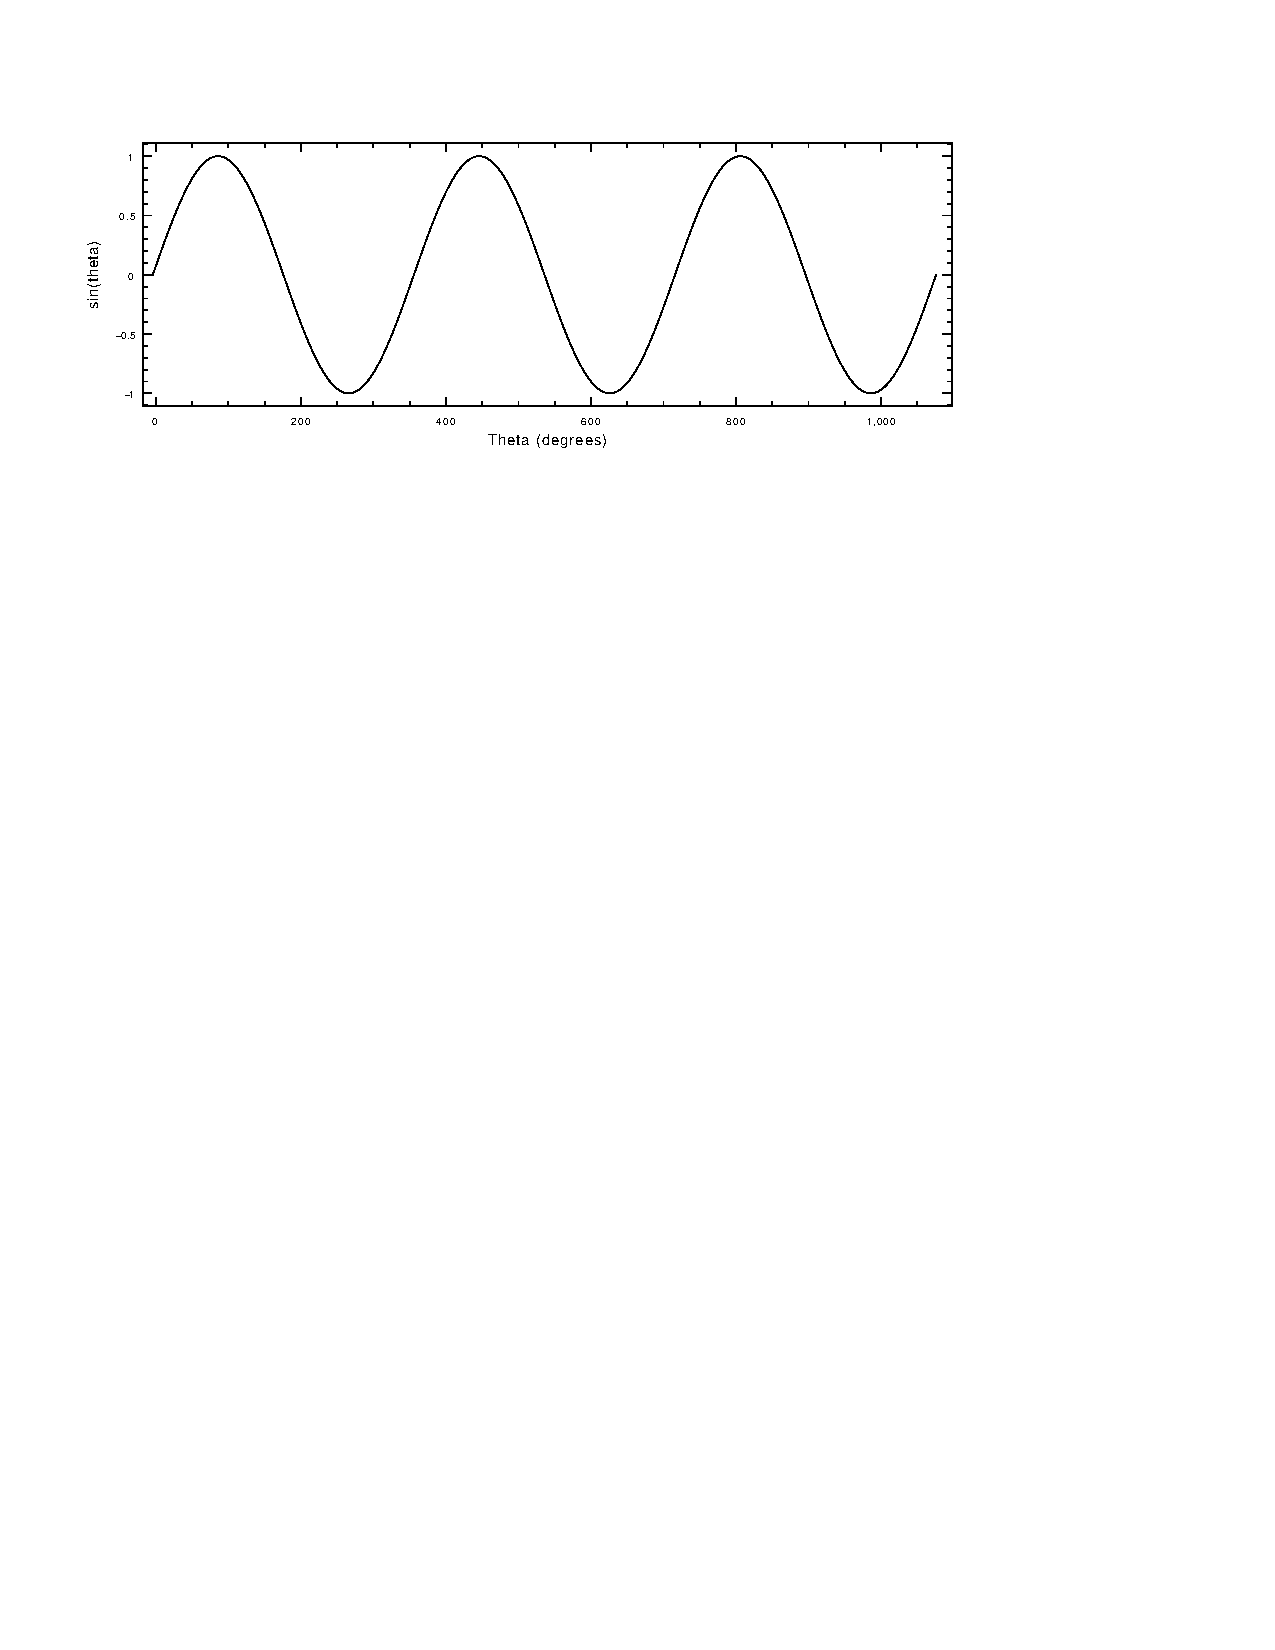
\includegraphics[width=5.5in, trim=0.5in 8.0in 2.0in 0.8in, clip]{sine_plot.pdf}
\caption{The sine curve.}
\label{fig_sine_plot}
\end{figure}

So far we have been measuring angles in degrees, but degrees are pretty
arbitrary units. The only reason there are 360 degrees in a circle is
that 360 is a nice round number that is close to the number of days in
a year. We should pick units that are more ``natural''. We will explain
why later, but the ``natural'' units for angles are radians. Radians are defined as the lengh of an arc divided by its radius. So in some sense they
are unitless, and therefore more ``mathy'' than the arbitrarily defined
degrees. If you have ever computed the sine in a program, then you know
that the \code{sin} function takes its argument in radians in essentially
every programming language. There are $2\pi$ radians in a circle, so you
convert from degrees to radians by multiplying by $\pi/180$.
From now on whenever we refer to the sine function, it its argument
will be measured in radians.

We introduced the sine function in terms of its geometric interpretation,
but from now on we will just think of it as a function. You won't see
another triangle for the rest of this book.

Now consider the following:
\begin{equation}
y = A\sin(\omega t + \phi)
\label{eq_omega}
\end{equation}
We added a few bells and whistles to the basic sine function. First we
multiplied it by $A$, so now instead of oscilating between $-1$ and $1$,
it oscilates between $-A$ and $A$. We call $A$ the ``amplitude'' of the
wave. Then we add $\phi$ to the argument. This shifts the wave to the right.
We call this the $phase$ of the wave. For what it's worth, if $\phi = \pi/2$
radians ($90^\circ$), then we have the cosine function. If $\phi = \pi$
($180^\circ$), then we have flipped the wave upside down. Finally, 
$\omega$ changes how fast the wave oscilates. If $\omega=1$ then we have one full cycle between $t=0$ and $t=2\pi$. If $\omega=2$, then we have
two cycles in the same interval.

So $\omega$ tells us about the frequency of the wave --- \ie how frequently
it goes through a cycle. Frequency comes in many flavors, so we need to 
be a little more specific. Suppose our sine wave describes the current in
a wire as a function of time. Then the ``frequency'' is the number of 
full cycles that happen in a second:
\begin{equation}
I = A sin(\frac{2\pi}{f} t + \phi)
\end{equation}
where $I$ is the current,
$t$ is time in seconds and $f$ is the frequency. 
The units of frequency are cycles per second, also known as ``Hertz'',
abbreviated ``Hz''.
The $\omega$ in Equation~\ref{eq_omega} is known as the ``angular frequency''.
It $t$ is in seconds, then it has units of radians per second.

Now suppose our sine wave describes a series of sand dunes in the Sahara
Desert. The distance between one wave peak and the next is known as the
``wavelength''. If $x$ is distance in meters, then
\begin{equation}
h = A sin(\frac{2\pi}{\lambda}x + \phi)
\end{equation}
where $h$ is the height of the dune, and
$\lambda$ is the wavelength in meters.

But wait, there's more. In some fields, people refer to the
``wave number'', defined as $1/\lambda$ and with units of 
${\rm meters}^{-1}$. There is also the ``angular wave number'', which is
$2\pi/\lambda$, with units of radians per meter. Just to be comfusing,
is is customary to use $k$ to refer to either of these.